\documentclass[../main.tex]{subfiles}

% Importing images from another path
\graphicspath{{\subfix{../images/}}}

\begin{document}

In this section, the collected latency data and the results obtained with the two implemented models are presented. As explained in section~\ref{architecture}, all the measurements have been repeated for multiple message sizes and the models have been trained accordingly. Although a clear relationship between the message size and the latency has been observed and the models are able to deal with multiple message sizes, this study focuses on the connection between latency and number of processes, hence this section will only present results relative to message size $1$ B due to space constraints.
Moreover, for the sake of brevity, the values for the $R^2$ metric, used as measurement of goodness of the models, are available in appendix~\ref{appendix}.\\
Figure~\ref{fig:bcast-results} shows the results obtained for the different algorithms \textbf{broadcast} operation with all the possible mapping policies. 
As anticipated, the default algorithm has only been fitted with the linear model due to the impossibility of knowing the exact algorithm executed before runtime. The difference between the different mapping policies is significant in these three plots. As expected, the \cc{map-by core} plot shows $4$ distinct segments where the slope of the measured data changes corresponding to the allocation of a new socket in the underlying architecture. The same pattern repeats for the \cc{socket} allocation but in this case only one change is visible, logically correponding to a new node being allocated. The \cc{node} allocation, instead, shows a single slope as expected. Although not perfect, the linear model is able to predict with enough accuracy the latencies of all three allocations, with an $R^2$ being respectively $0.92$, $0.90$ and $0.89$, the only exception being the initial trend of the socket allocation that shows a seemingly logarithmic trend.\\
Regarding the linear algorithm, the linear fit expectedly predicts with high accuracy the latencies in all of the three cases, but good results have also been obtained with the point-to-point model. The latter, in fact, is able to predict seemingly perfectly the initial trends of the core and socket allocation, while showing slight over/under-estimations for the final part of the plots and for the node allocation.\\
Similar results have been obtained for the chain algorithm, where the point-to-point model predicts almost perfectly the measured latencies up to the first node, but the underestimates the latencies when a second node starts being allocated in the core and socket cases. Here again, the linear fit turns out to be the superior model in terms of accuracy.\\
Concerning the binary tree algorithm, the logarithmic trend hypotesized in the previous section is confirmed by the measured data. However, this is only true in the case of the node allocation and for the initial part of the plot in the core and socket cases. In fact, when the second node starts being allocated, the latencies start to increment almost linearly with $P$. For this reason the predictions of the point-to-point model only match the measured data up to the first node, while the linear model has been modified to fit and initial logarithmic trend, plus a final linear trend in those cases, showing the versatility of this model.\\
Figure~\ref{fig:reduce-results} then shows the results obtained for the \textbf{reduce} operation. In the case of the default algorithm, worse results are obtained by the linear fit in the case of the core allocation with respect to those obtained in the cases of the socket and node allocation, mostly due to the absence of an evident linear trend in the first case.\\
In the case of the linear algorithm, the measured data for the core and socket mappings showed a strange behavior where an initial expected linear trend up to the first node is then followed by a decrease in latency for increasing number of processes in the second node. The linear model is of course able to fit the data anyway but the phenomenon is not easily explainable, suggesting the more probable possibility of anomalies in the measurement process. The node allocation, instead, shows a clear linear trend that is perfectly fitted by the linear model. However, the point-to-point model completely fails to allign predictions with measured data in this cases, the only exception being the latecies measured for the first socket in the core allocation. Again, this can be due to anomalies in the measurement process, particularly in the measurements of the NBFT latencies for the estimation of $\gamma^{c}$ as explained in section~\ref{architecture}.\\
Finally, both the chain and binary tree algorithms present the same aspects obseerved for the broadcast operation with slight differences. The major one being the binary tree algorithm in the case of the node mapping, which does not show any logarithmic trend but rather almost constant and relatively small latency times for increasing numbers of $P$.\\

\begin{figure}[p]
    \begin{adjustwidth}{-1.5cm}{-1.5cm}
    \centering
    \begin{minipage}{0.40\textwidth}
        \centering
        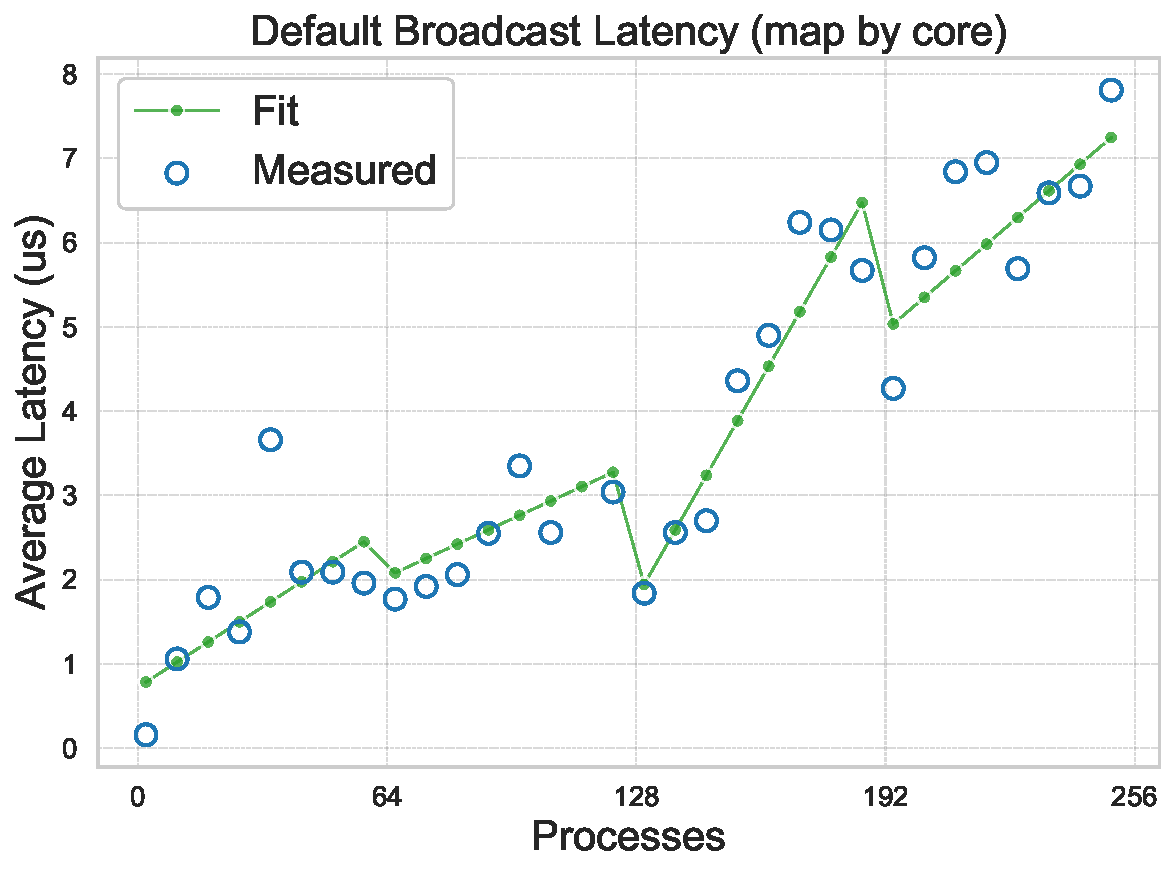
\includegraphics[width=\textwidth]{bcast-default-core.pdf}
    \end{minipage}\hfill
    \begin{minipage}{0.40\textwidth}
        \centering
        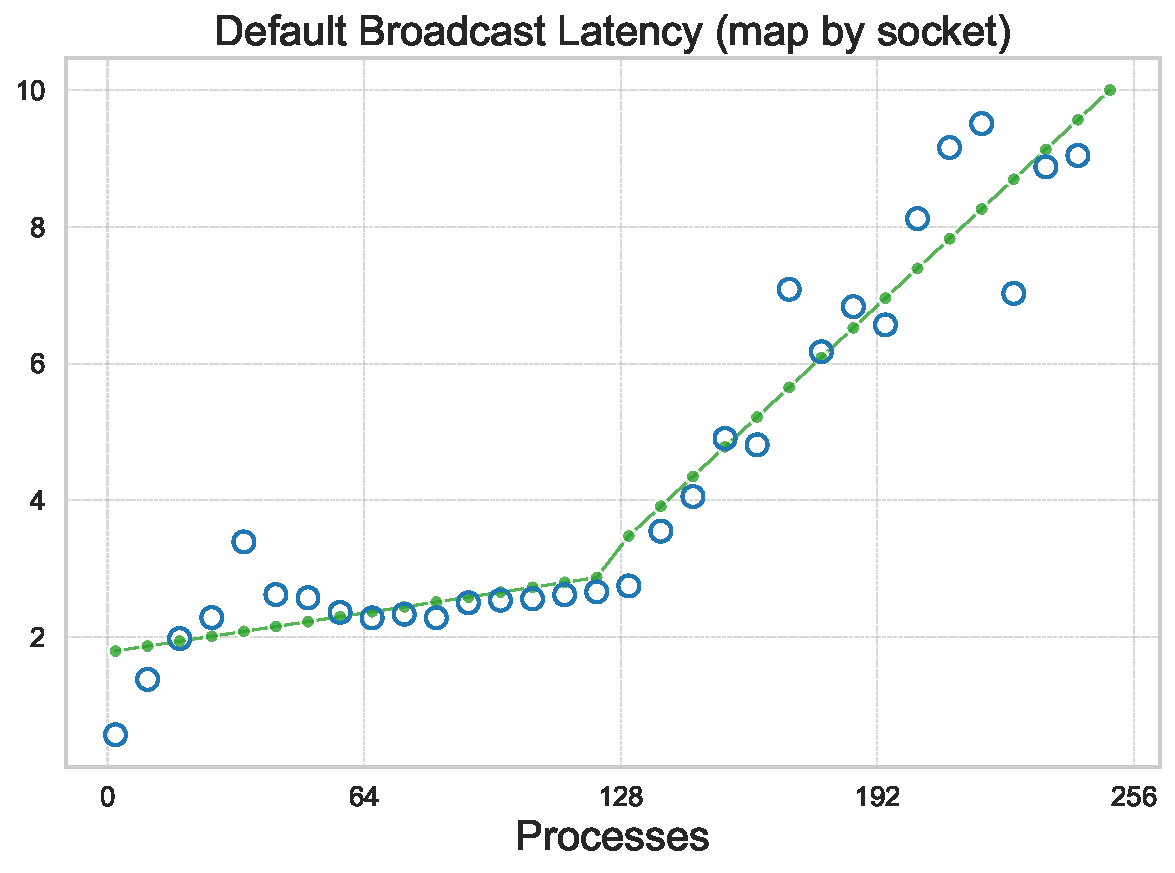
\includegraphics[width=\textwidth]{bcast-default-socket.pdf}
    \end{minipage}\hfill
    \begin{minipage}{0.40\textwidth}
        \centering
        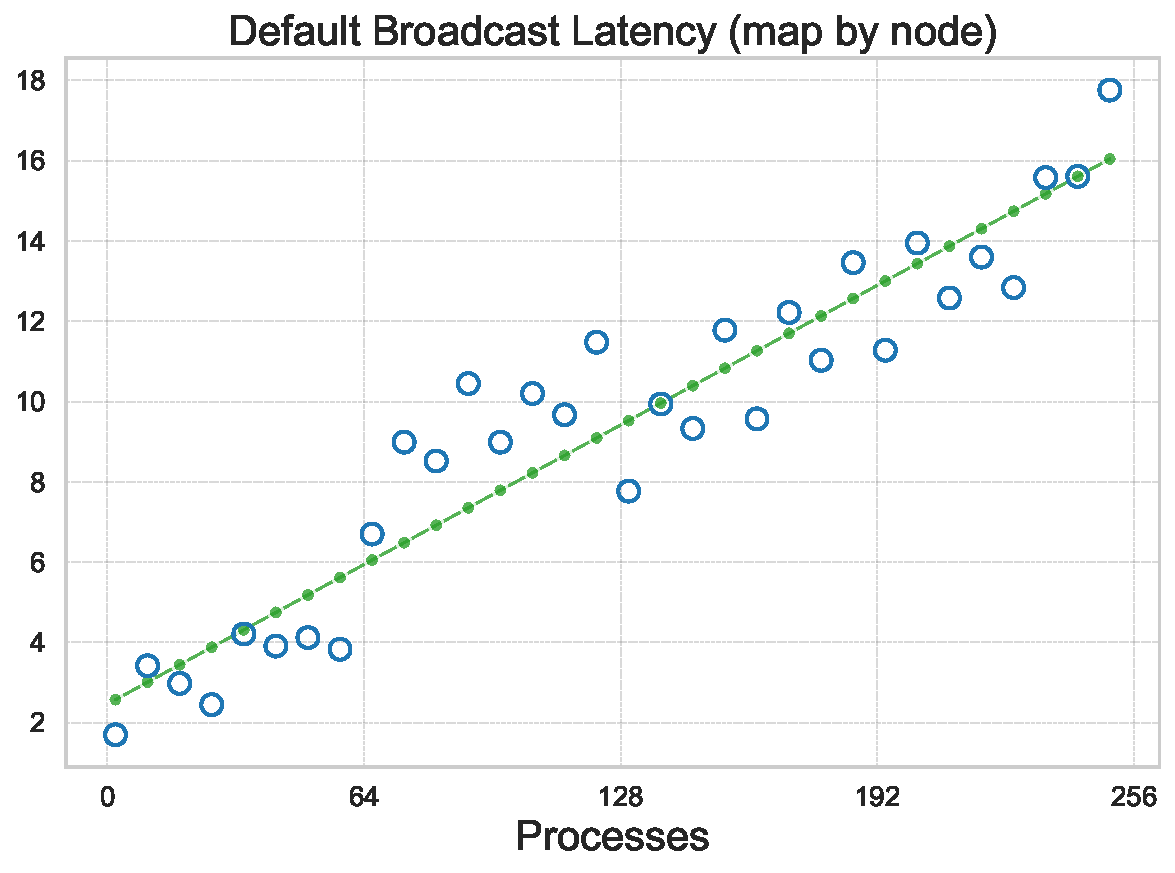
\includegraphics[width=\textwidth]{bcast-default-node.pdf}
    \end{minipage}
    \begin{minipage}{0.40\textwidth}
        \centering
        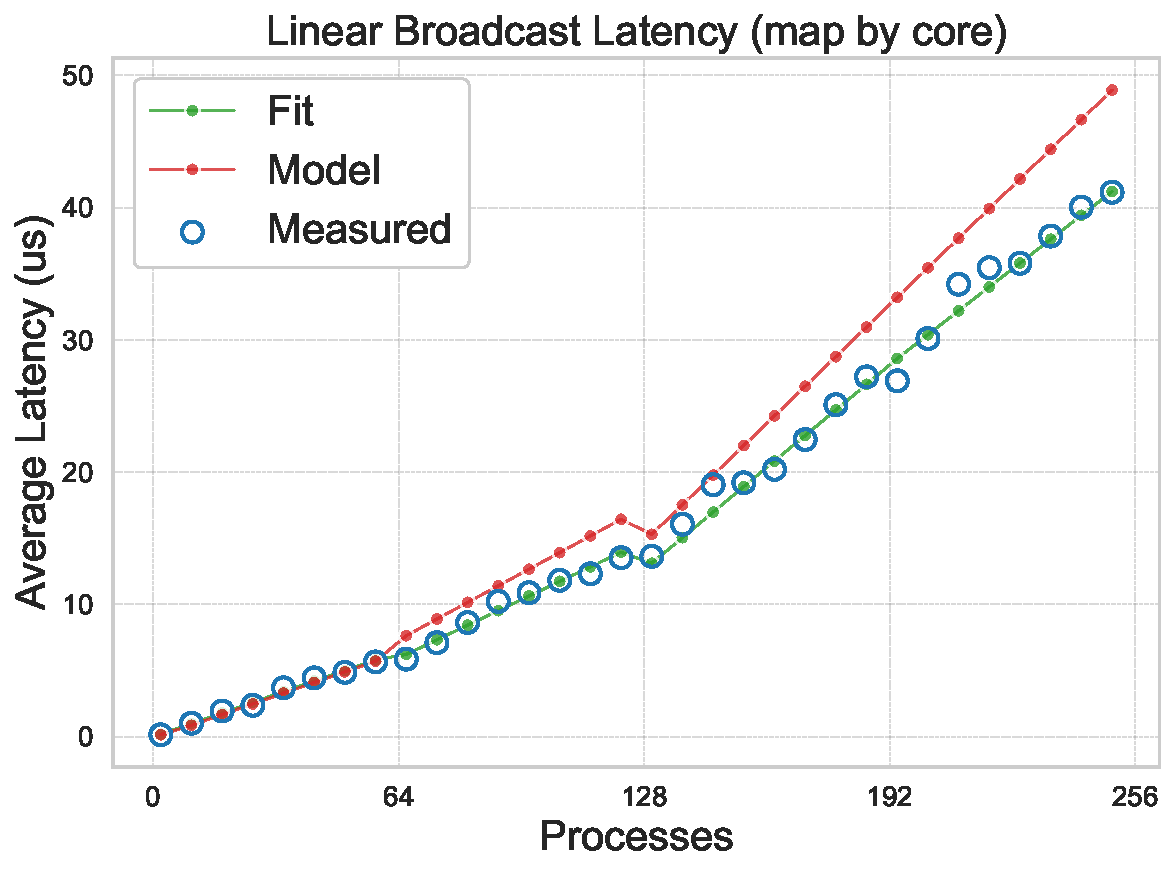
\includegraphics[width=\textwidth]{bcast-linear-core.pdf}
    \end{minipage}\hfill
    \begin{minipage}{0.40\textwidth}
        \centering
        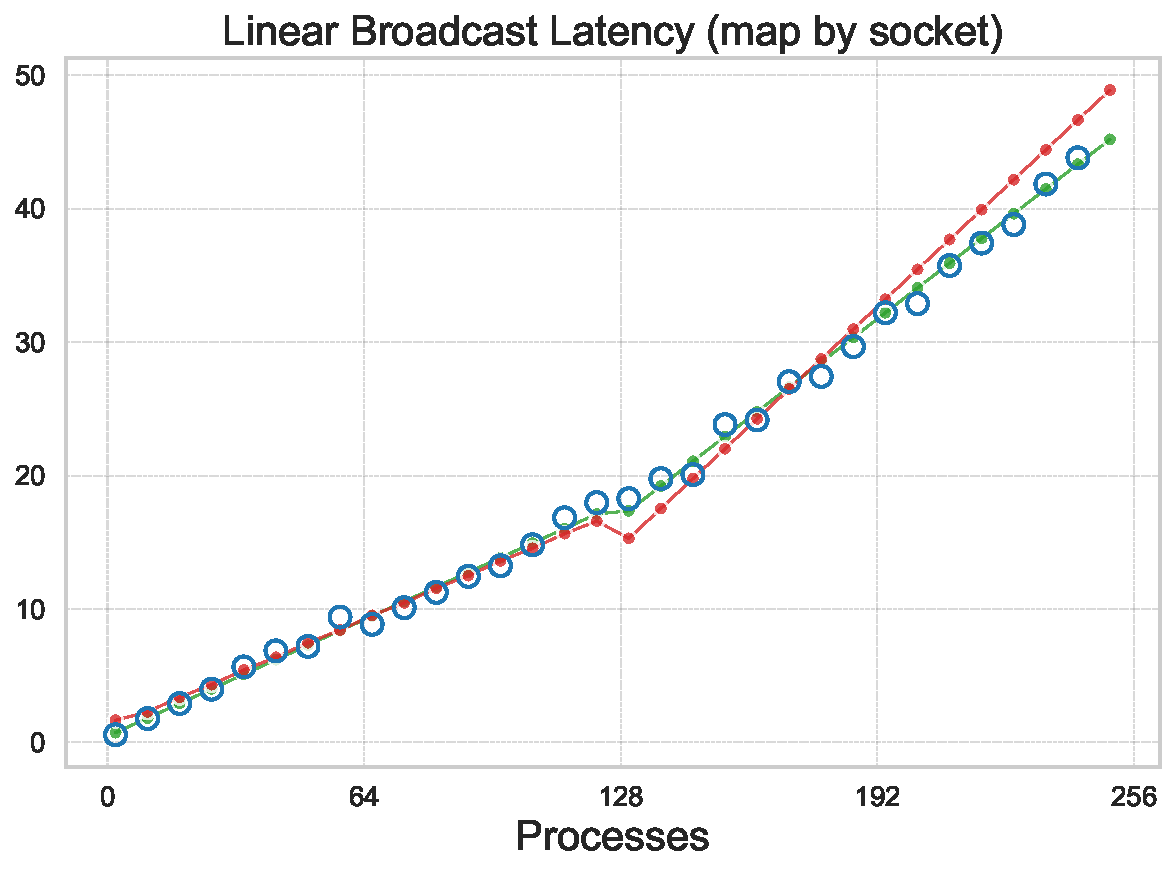
\includegraphics[width=\textwidth]{bcast-linear-socket.pdf}
    \end{minipage}\hfill
    \begin{minipage}{0.40\textwidth}
        \centering
        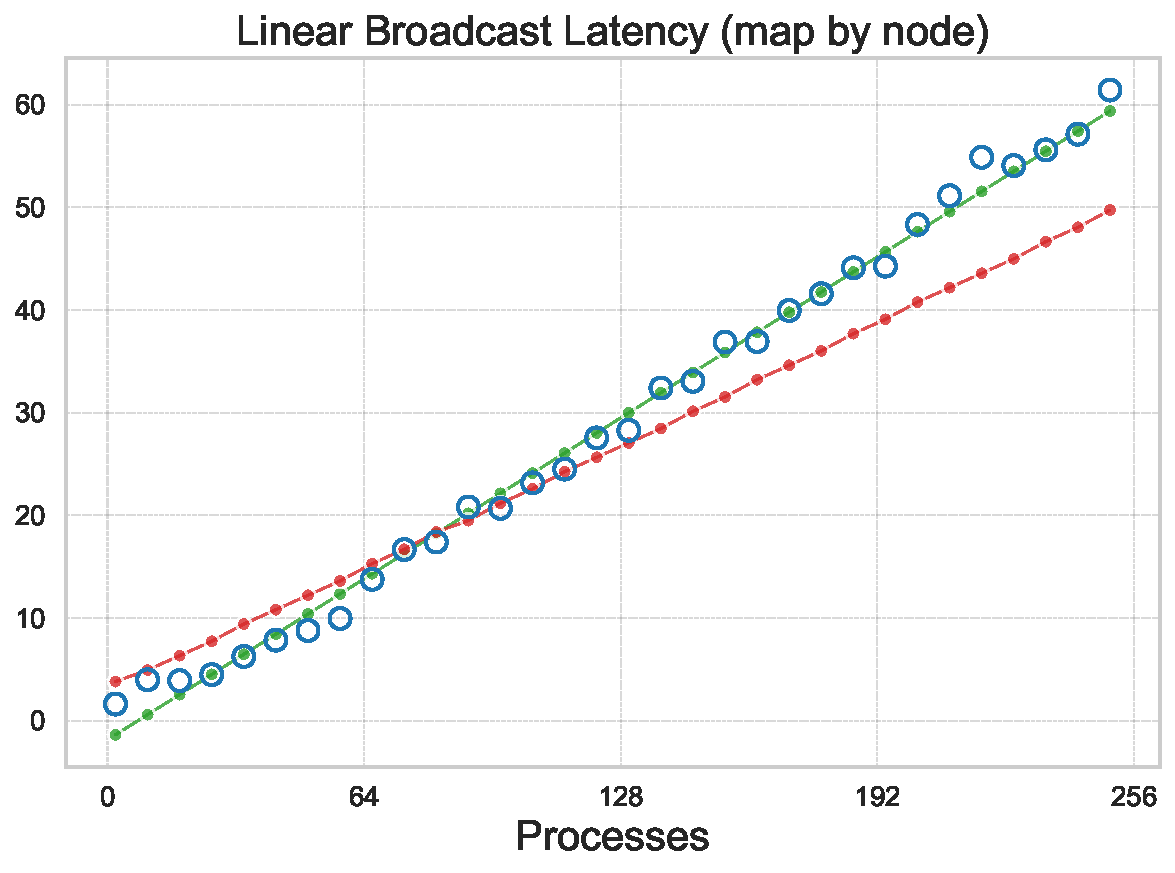
\includegraphics[width=\textwidth]{bcast-linear-node.pdf}
    \end{minipage}
    \begin{minipage}{0.40\textwidth}
        \centering
        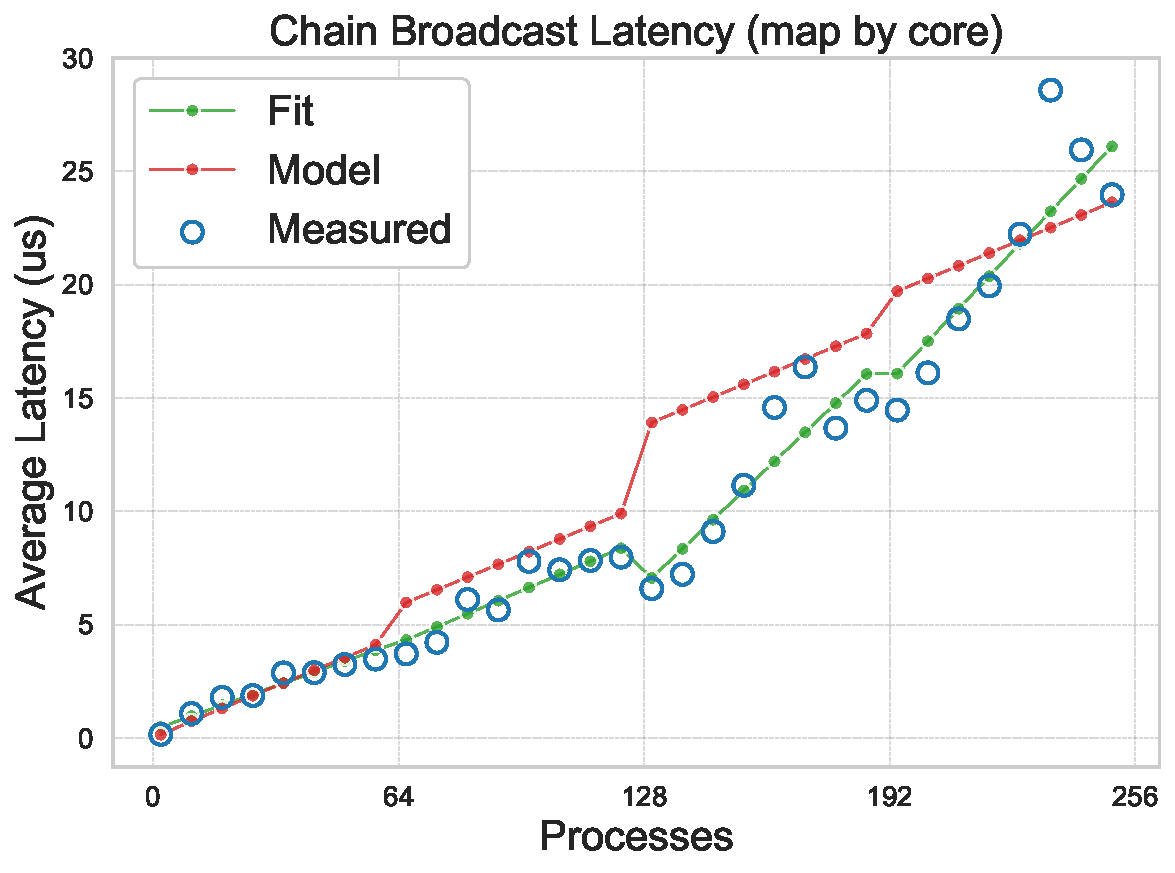
\includegraphics[width=\textwidth]{bcast-chain-core.pdf}
    \end{minipage}\hfill
    \begin{minipage}{0.40\textwidth}
        \centering
        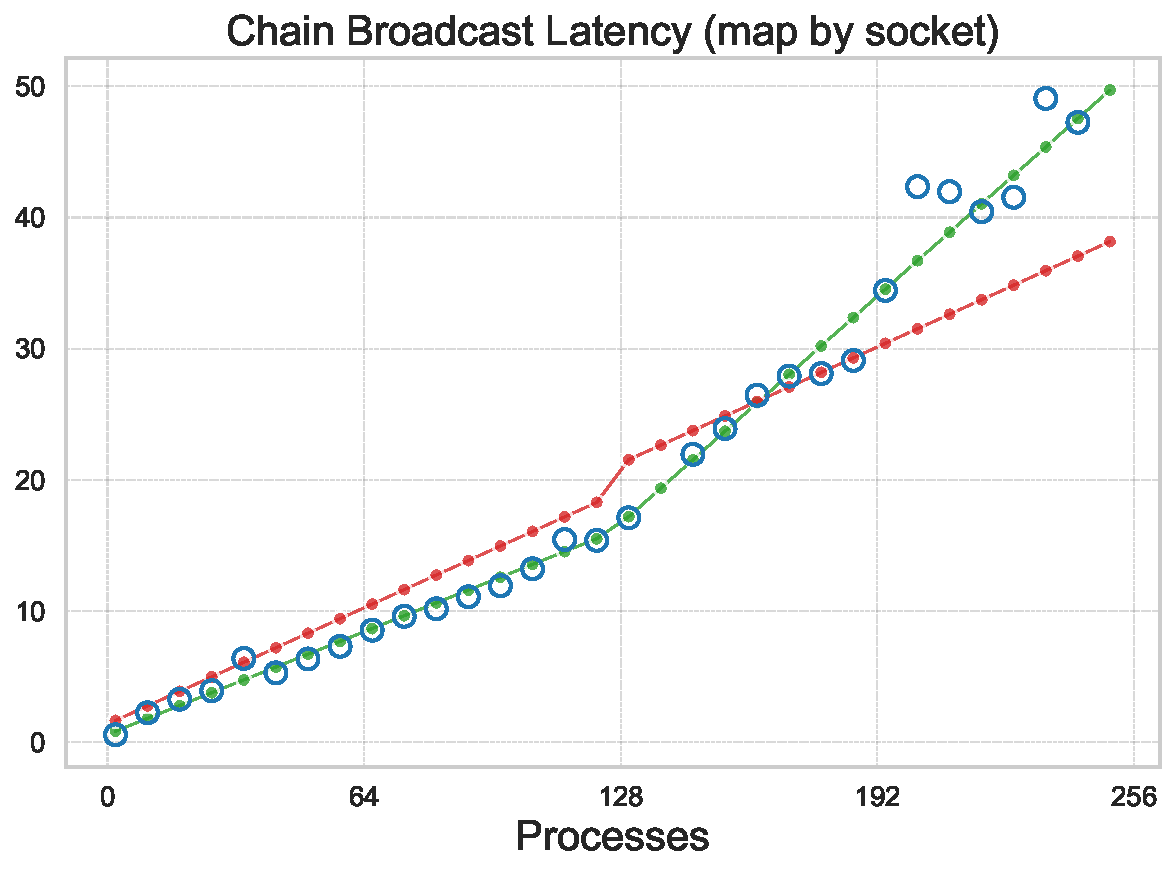
\includegraphics[width=\textwidth]{bcast-chain-socket.pdf}
    \end{minipage}\hfill
    \begin{minipage}{0.40\textwidth}
        \centering
        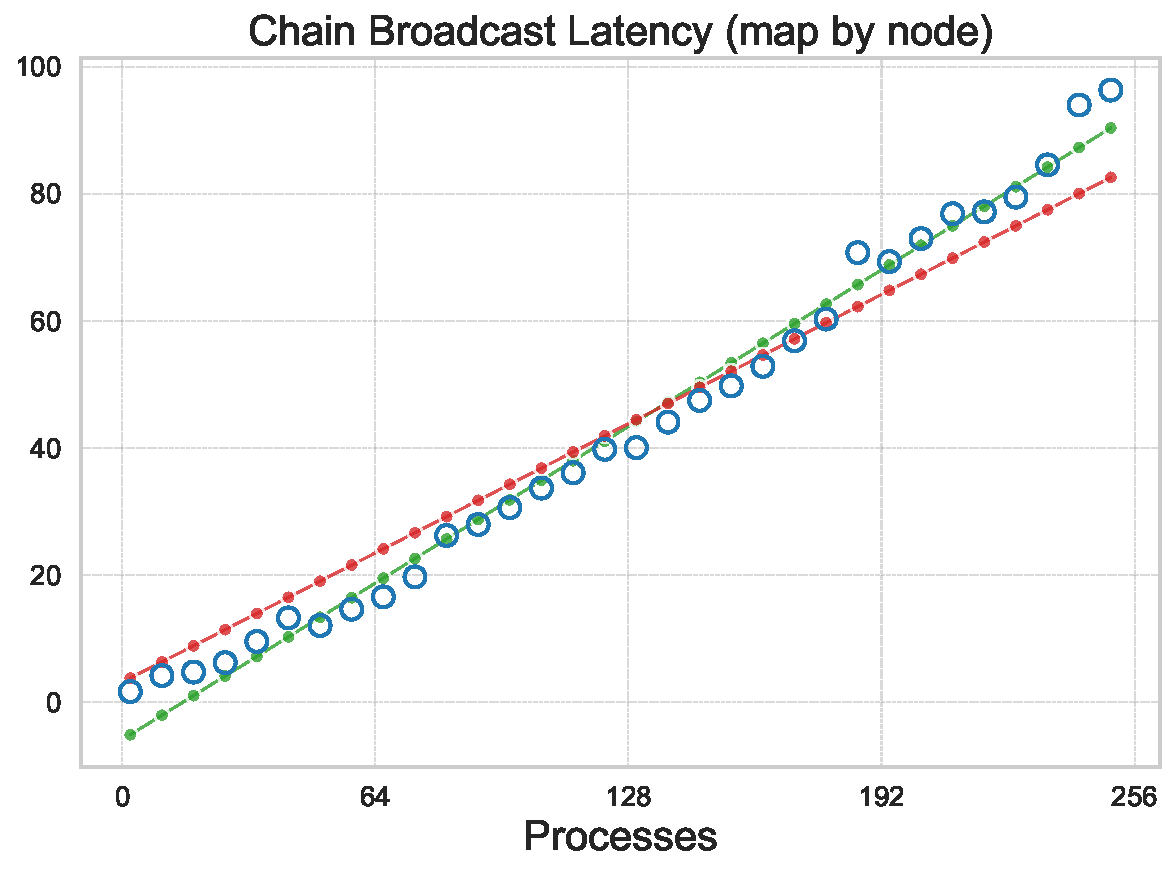
\includegraphics[width=\textwidth]{bcast-chain-node.pdf}
    \end{minipage}
    \begin{minipage}{0.40\textwidth}
        \centering
        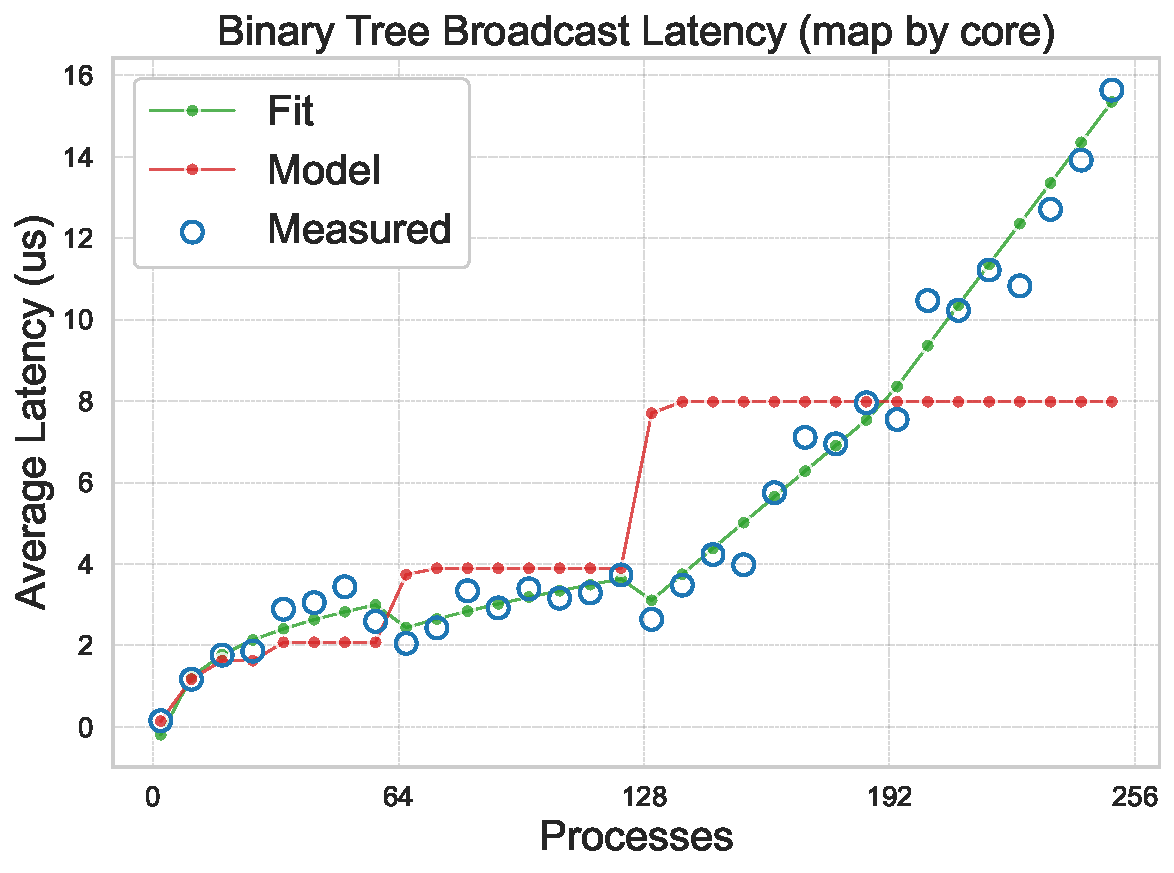
\includegraphics[width=\textwidth]{bcast-binary-core.pdf}
    \end{minipage}\hfill
    \begin{minipage}{0.40\textwidth}
        \centering
        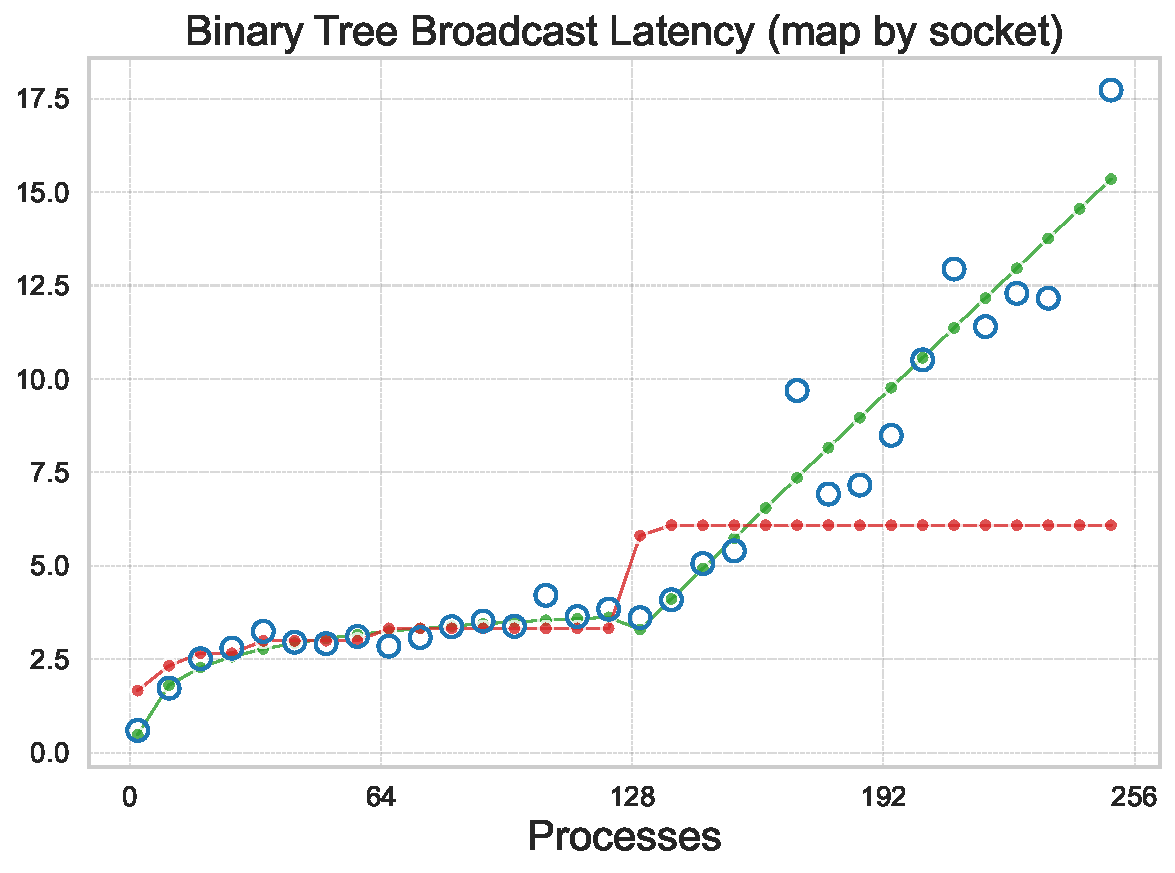
\includegraphics[width=\textwidth]{bcast-binary-socket.pdf}
    \end{minipage}\hfill
    \begin{minipage}{0.40\textwidth}
        \centering
        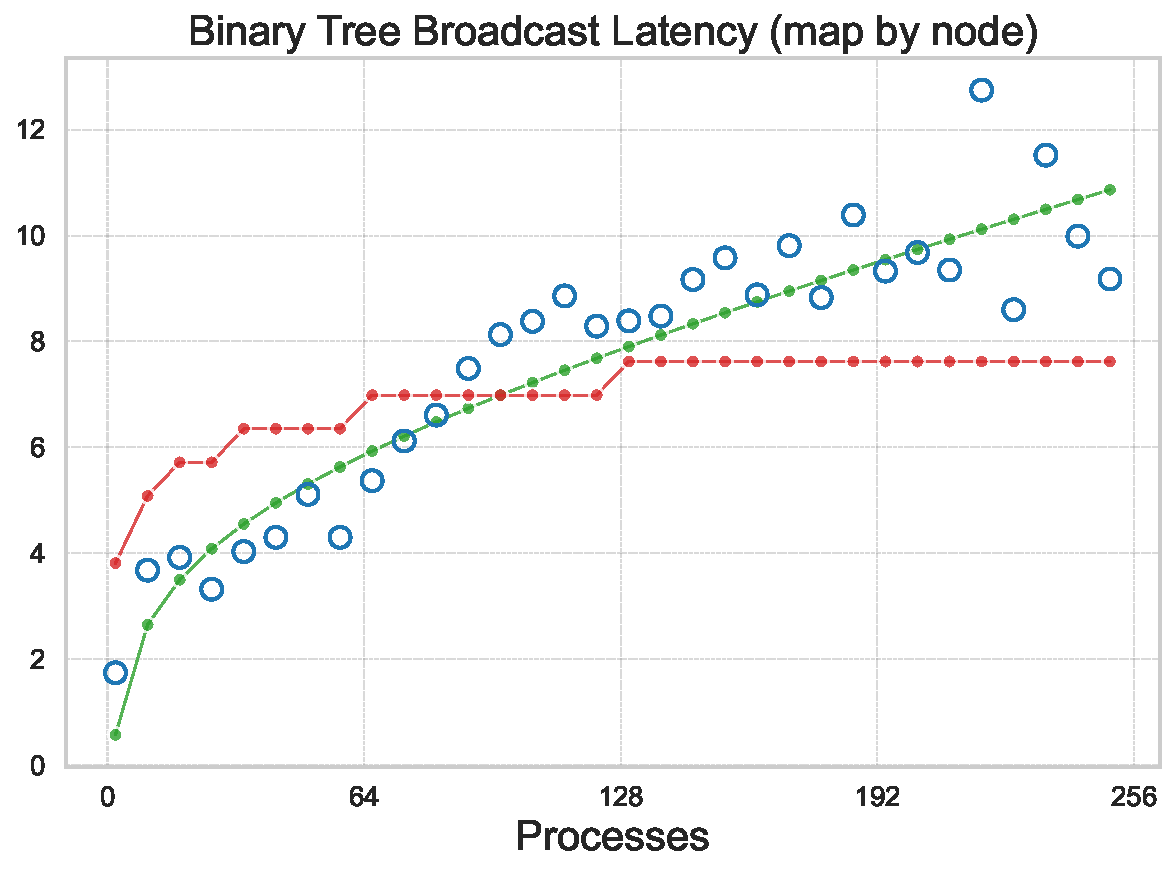
\includegraphics[width=\textwidth]{bcast-binary-node.pdf}
    \end{minipage}
    \end{adjustwidth}
    
    \caption{Comparison between point-to-point and linear fit models for different \textbf{broadcast} algorithms and mapping policies. In blue the measured data, corresponding to a message size of $1$ B. The point-to-point model predictions are shown in red while the linear model predictions are shown in green.}
    \label{fig:reduce-results}
\end{figure}

\begin{figure}[p]
    \begin{adjustwidth}{-1.5cm}{-1.5cm}
    \centering
    \begin{minipage}{0.40\textwidth}
        \centering
        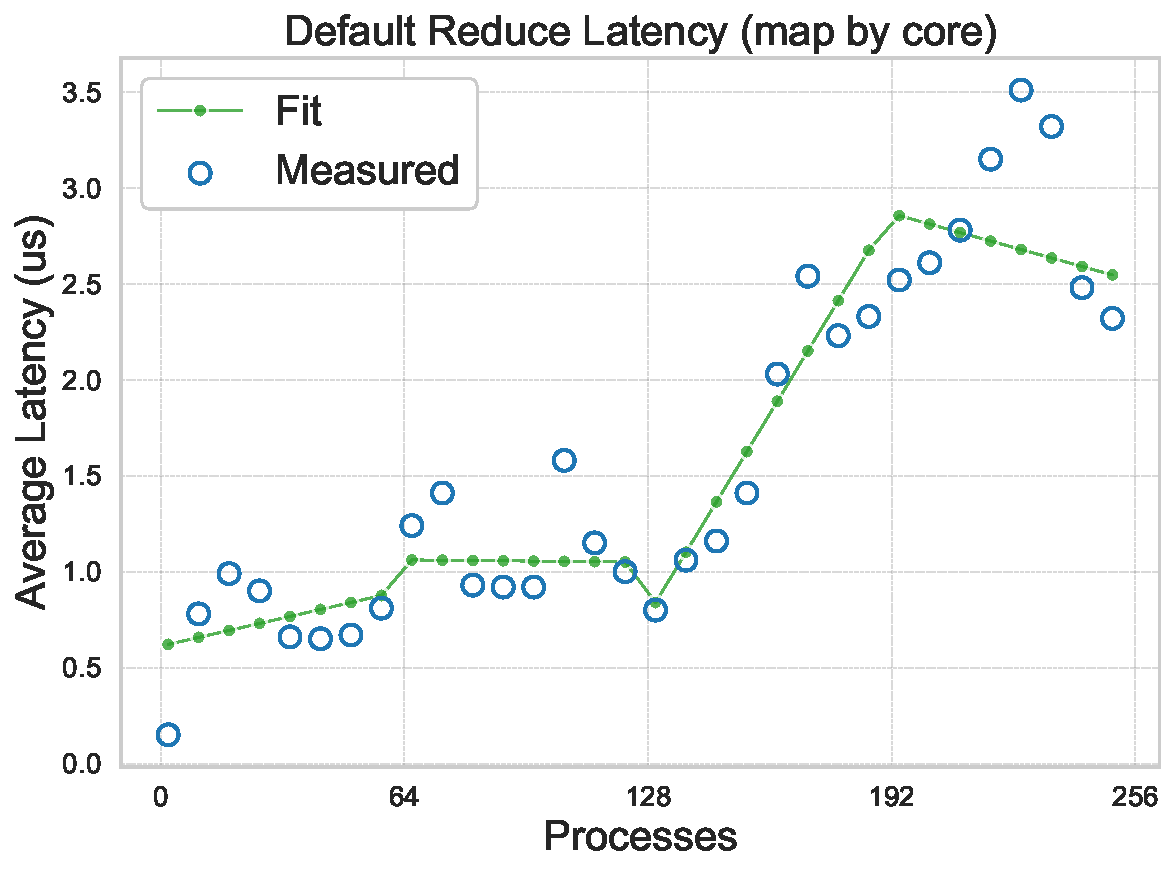
\includegraphics[width=\textwidth]{reduce-default-core.pdf}
    \end{minipage}\hfill
    \begin{minipage}{0.40\textwidth}
        \centering
        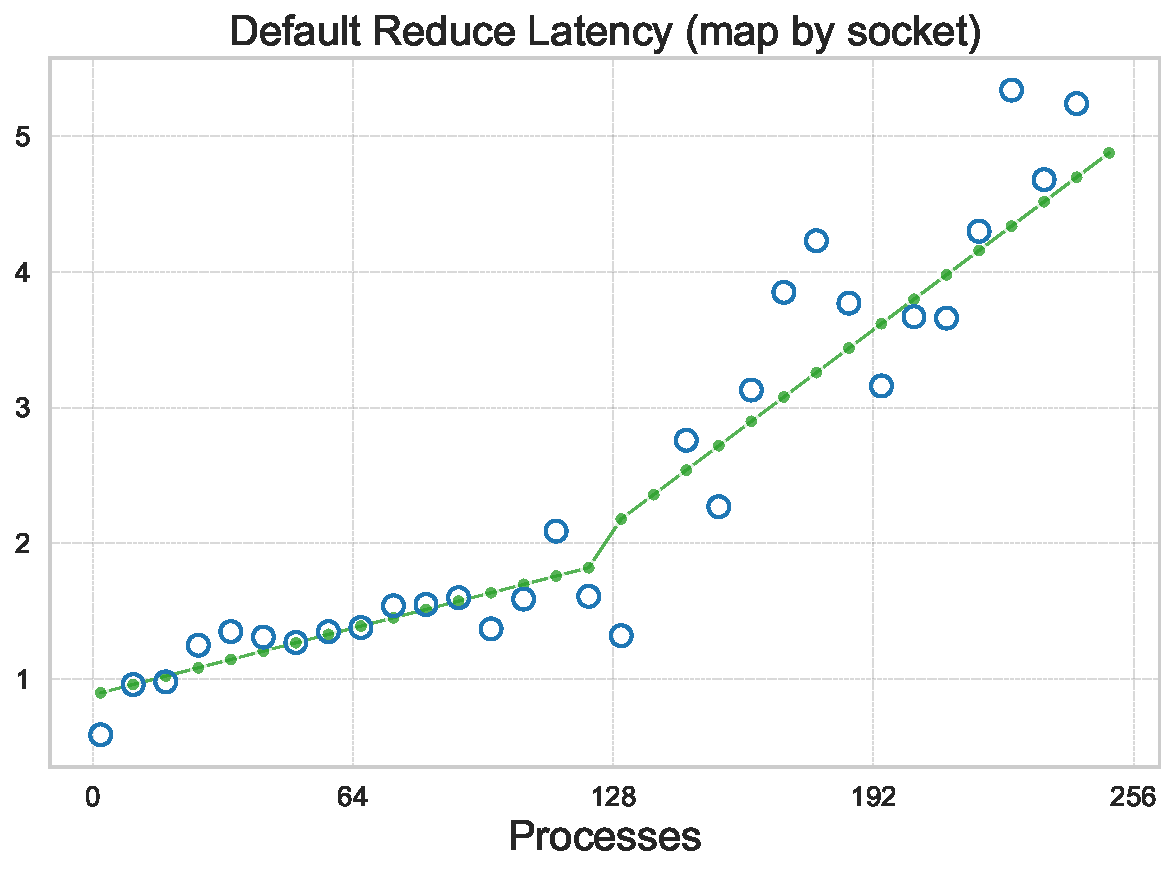
\includegraphics[width=\textwidth]{reduce-default-socket.pdf}
    \end{minipage}\hfill
    \begin{minipage}{0.40\textwidth}
        \centering
        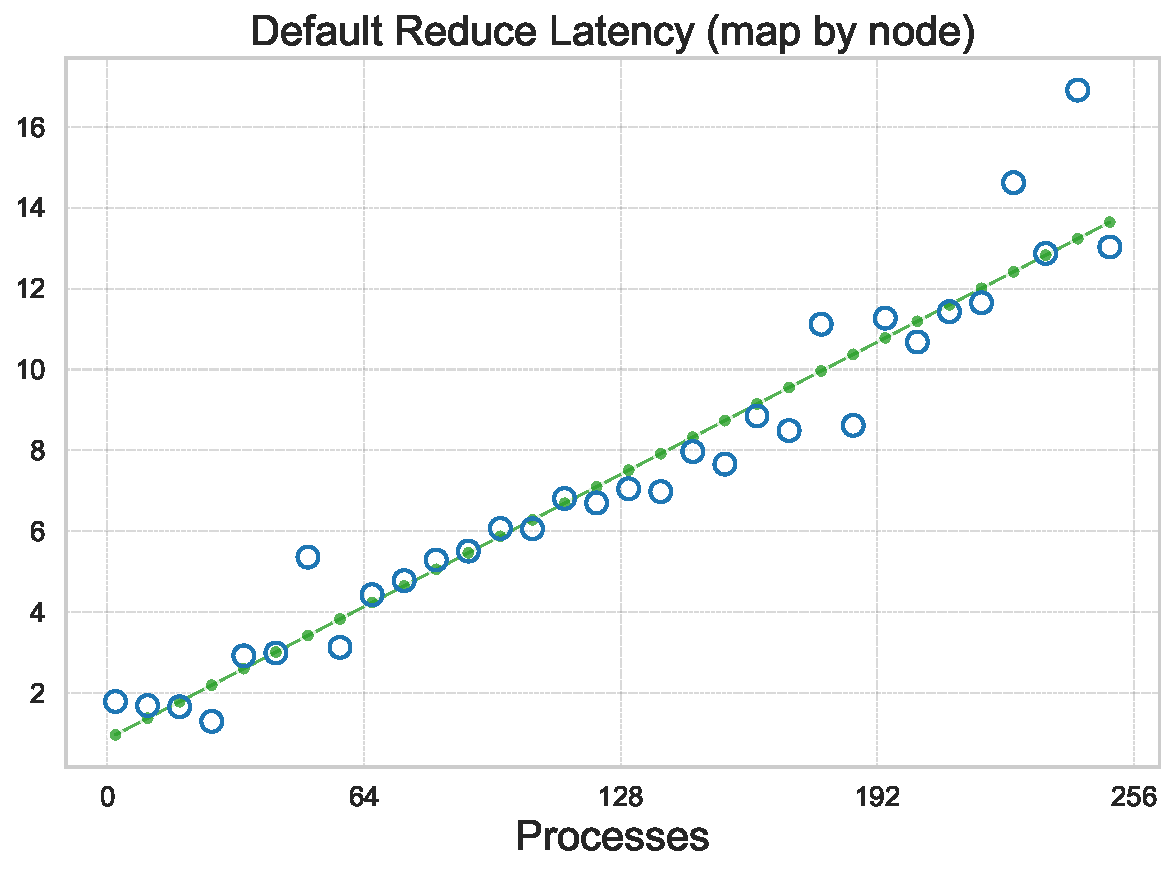
\includegraphics[width=\textwidth]{reduce-default-node.pdf}
    \end{minipage}
    \begin{minipage}{0.40\textwidth}
        \centering
        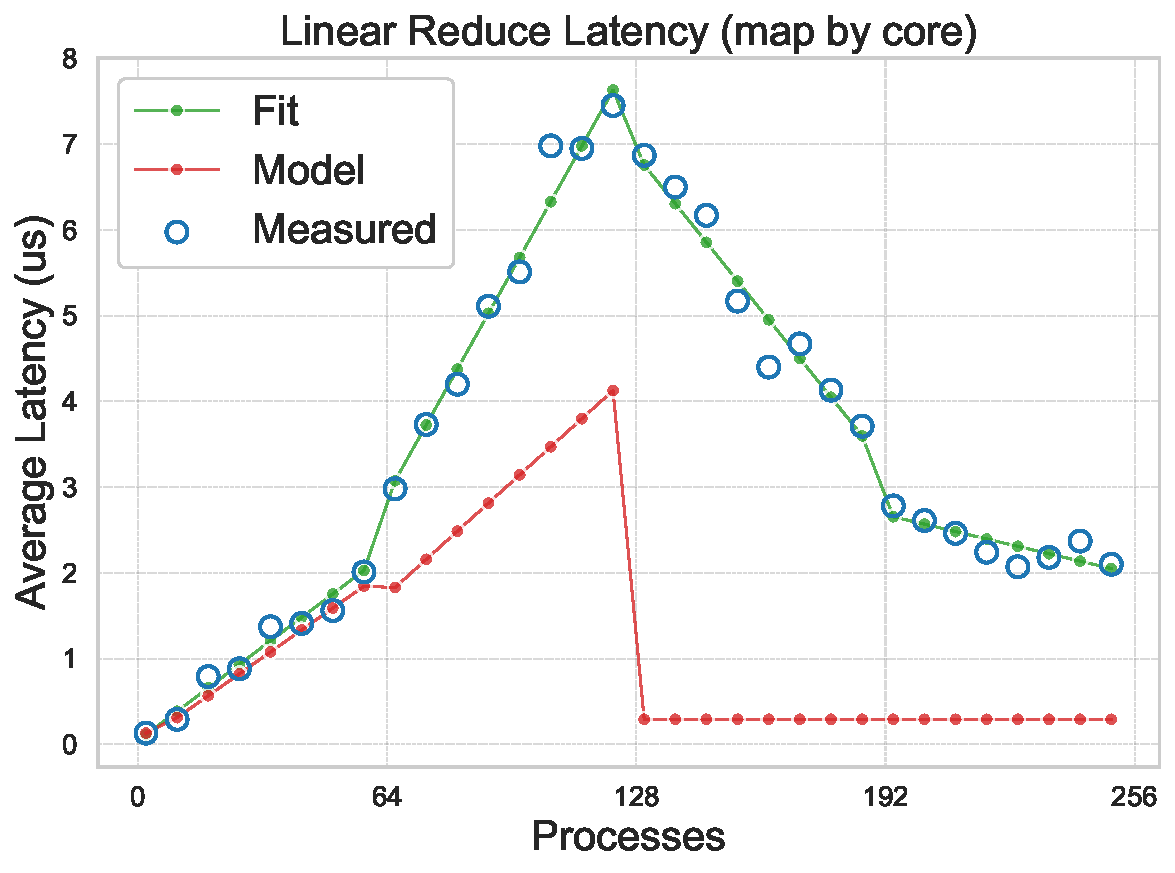
\includegraphics[width=\textwidth]{reduce-linear-core.pdf}
    \end{minipage}\hfill
    \begin{minipage}{0.40\textwidth}
        \centering
        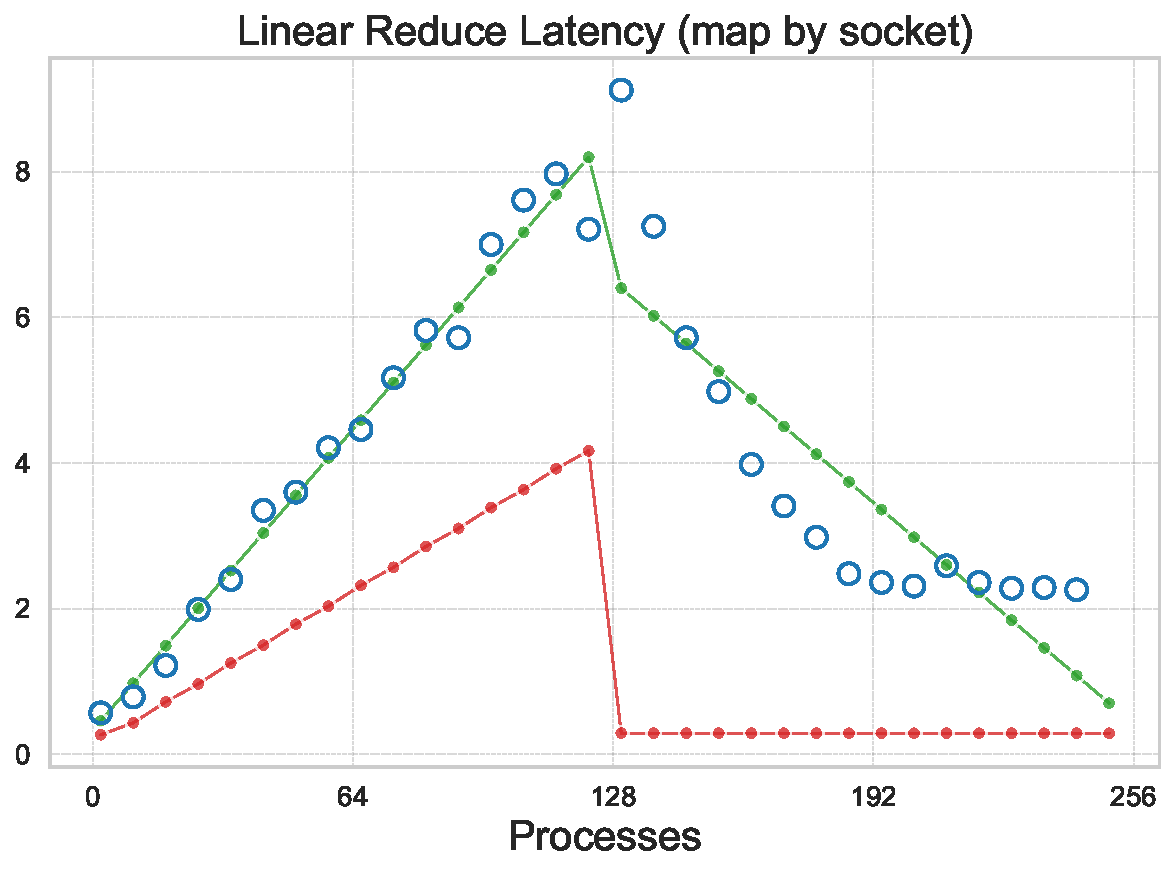
\includegraphics[width=\textwidth]{reduce-linear-socket.pdf}
    \end{minipage}\hfill
    \begin{minipage}{0.40\textwidth}
        \centering
        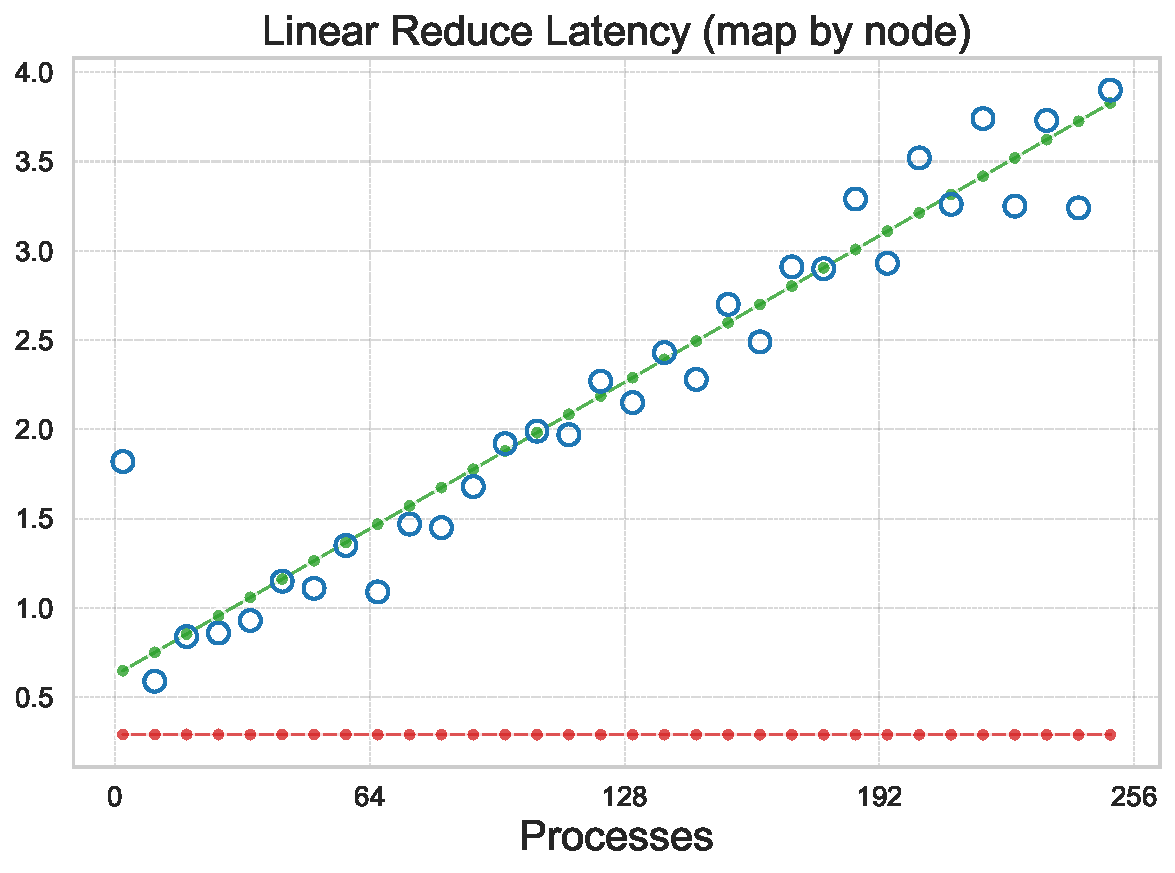
\includegraphics[width=\textwidth]{reduce-linear-node.pdf}
    \end{minipage}
    \begin{minipage}{0.40\textwidth}
        \centering
        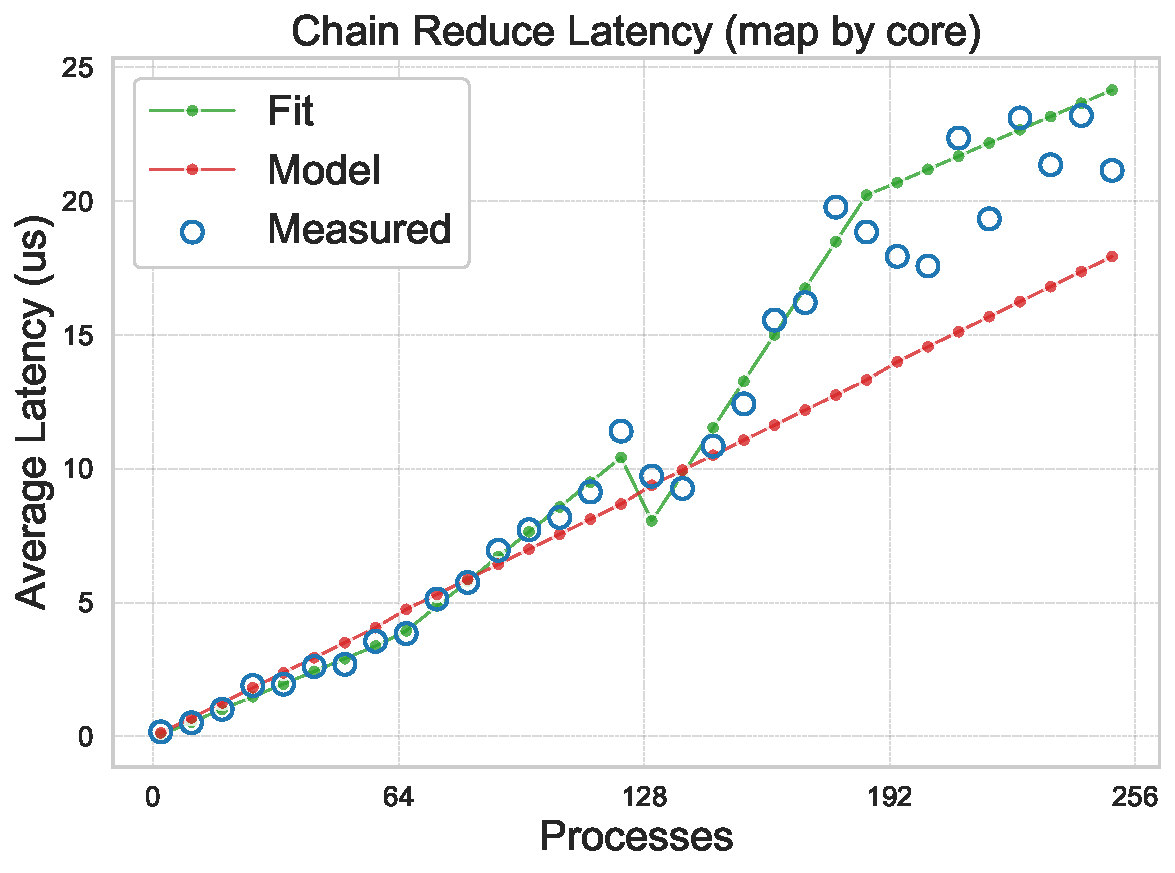
\includegraphics[width=\textwidth]{reduce-chain-core.pdf}
    \end{minipage}\hfill
    \begin{minipage}{0.40\textwidth}
        \centering
        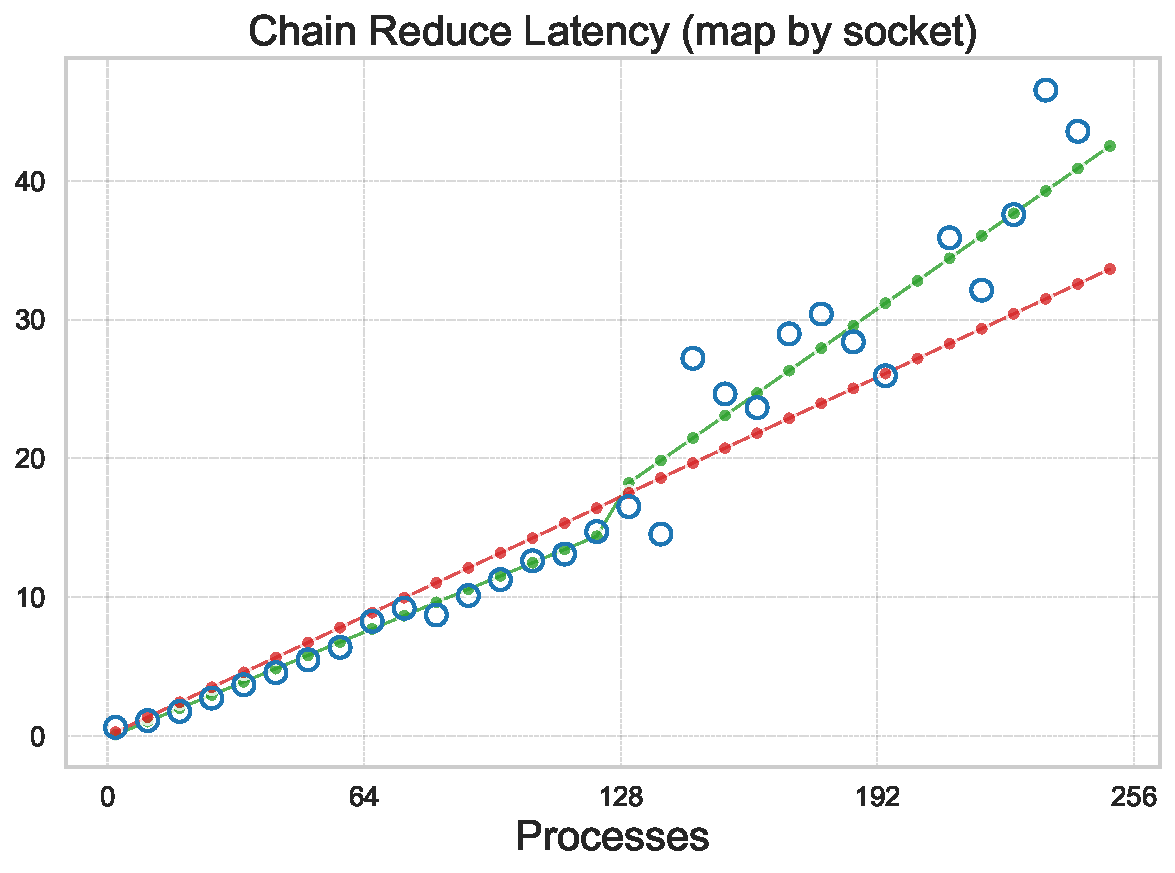
\includegraphics[width=\textwidth]{reduce-chain-socket.pdf}
    \end{minipage}\hfill
    \begin{minipage}{0.40\textwidth}
        \centering
        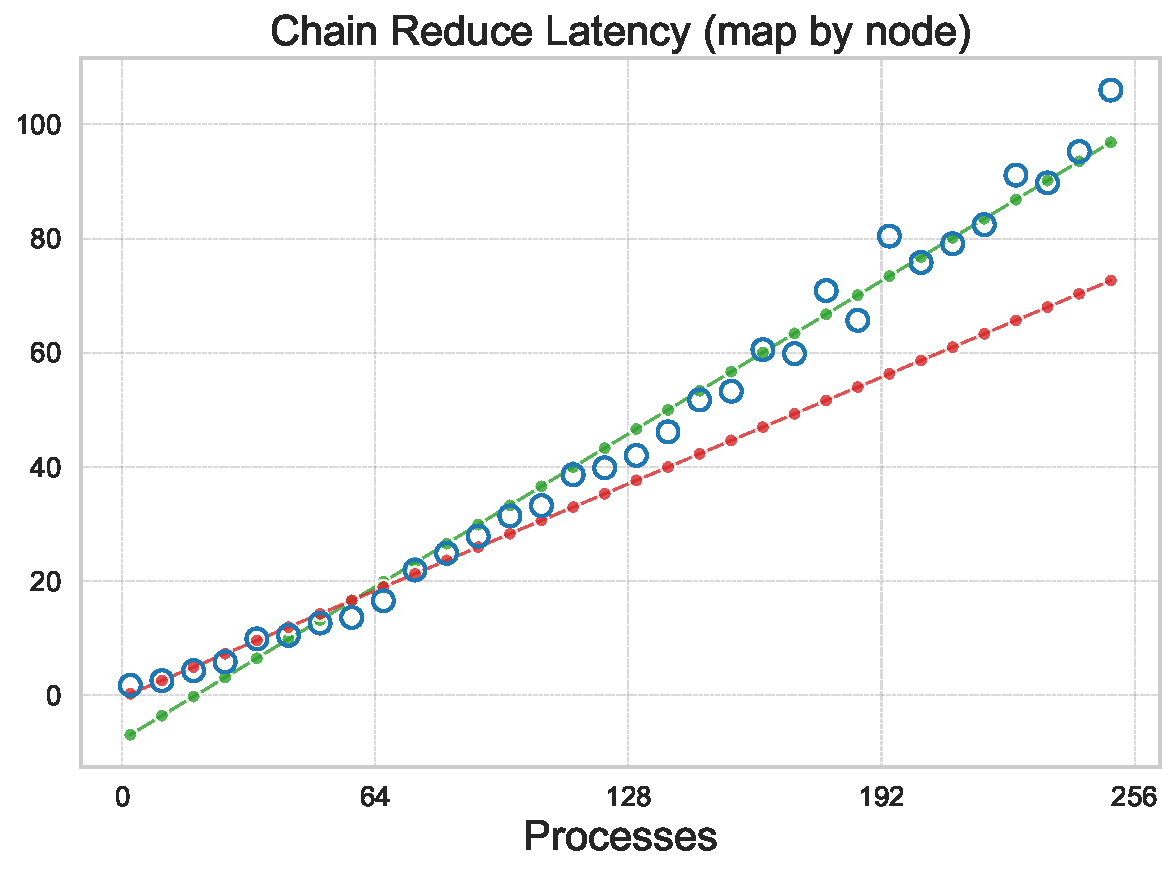
\includegraphics[width=\textwidth]{reduce-chain-node.pdf}
    \end{minipage}
    \begin{minipage}{0.40\textwidth}
        \centering
        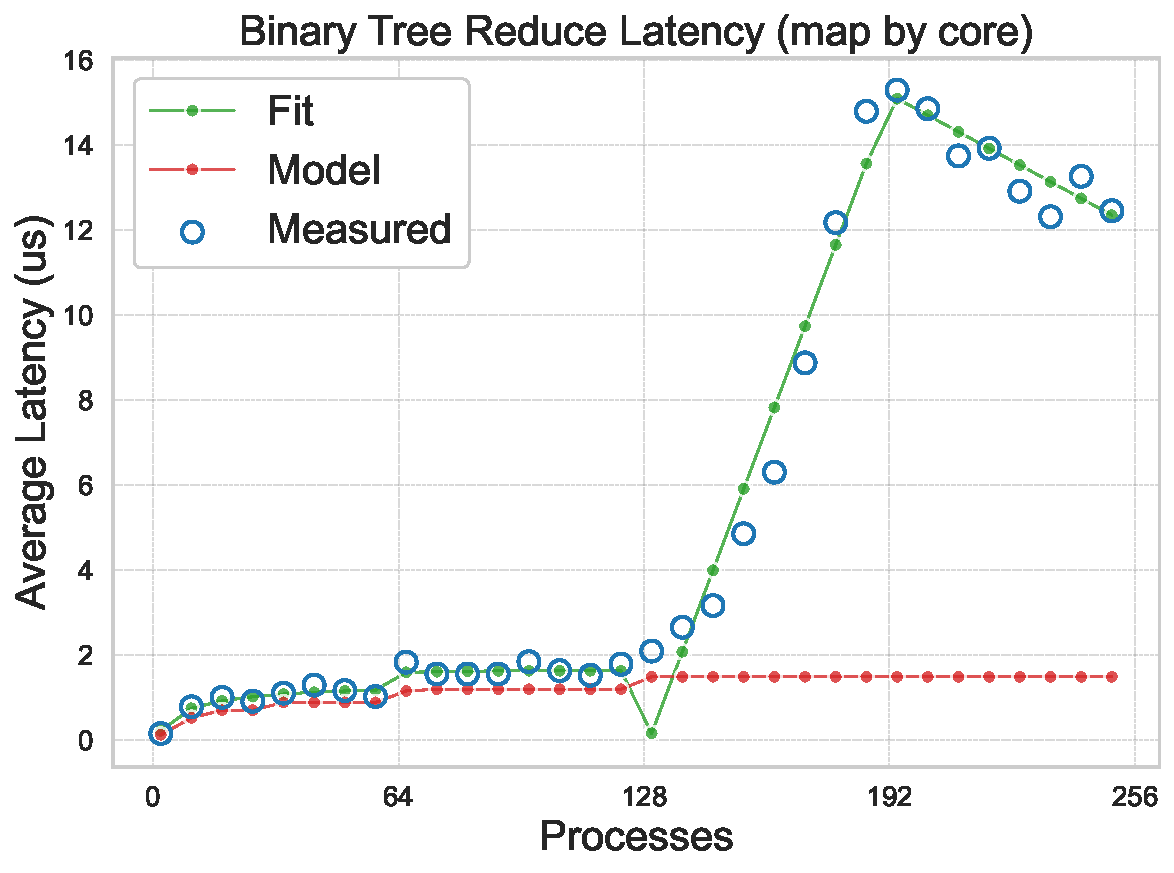
\includegraphics[width=\textwidth]{reduce-binary-core.pdf}
    \end{minipage}\hfill
    \begin{minipage}{0.40\textwidth}
        \centering
        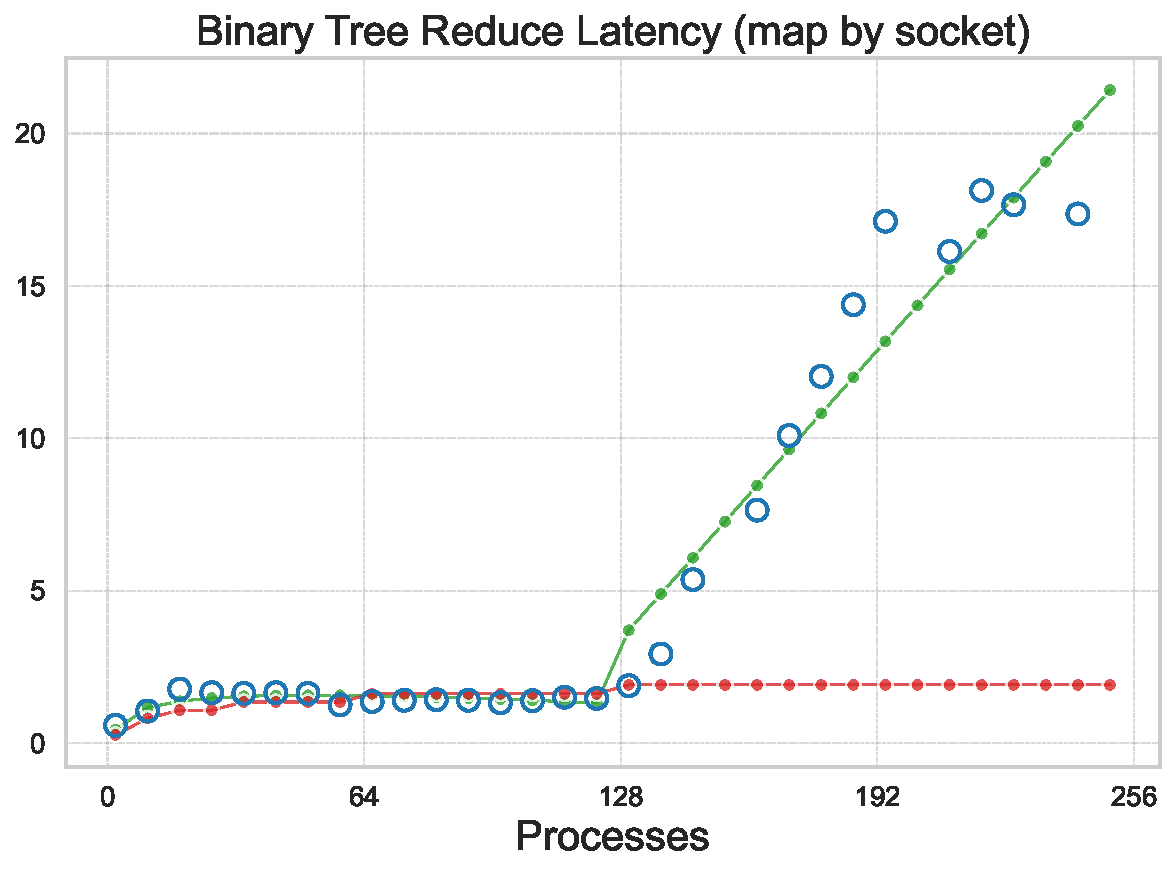
\includegraphics[width=\textwidth]{reduce-binary-socket.pdf}
    \end{minipage}\hfill
    \begin{minipage}{0.40\textwidth}
        \centering
        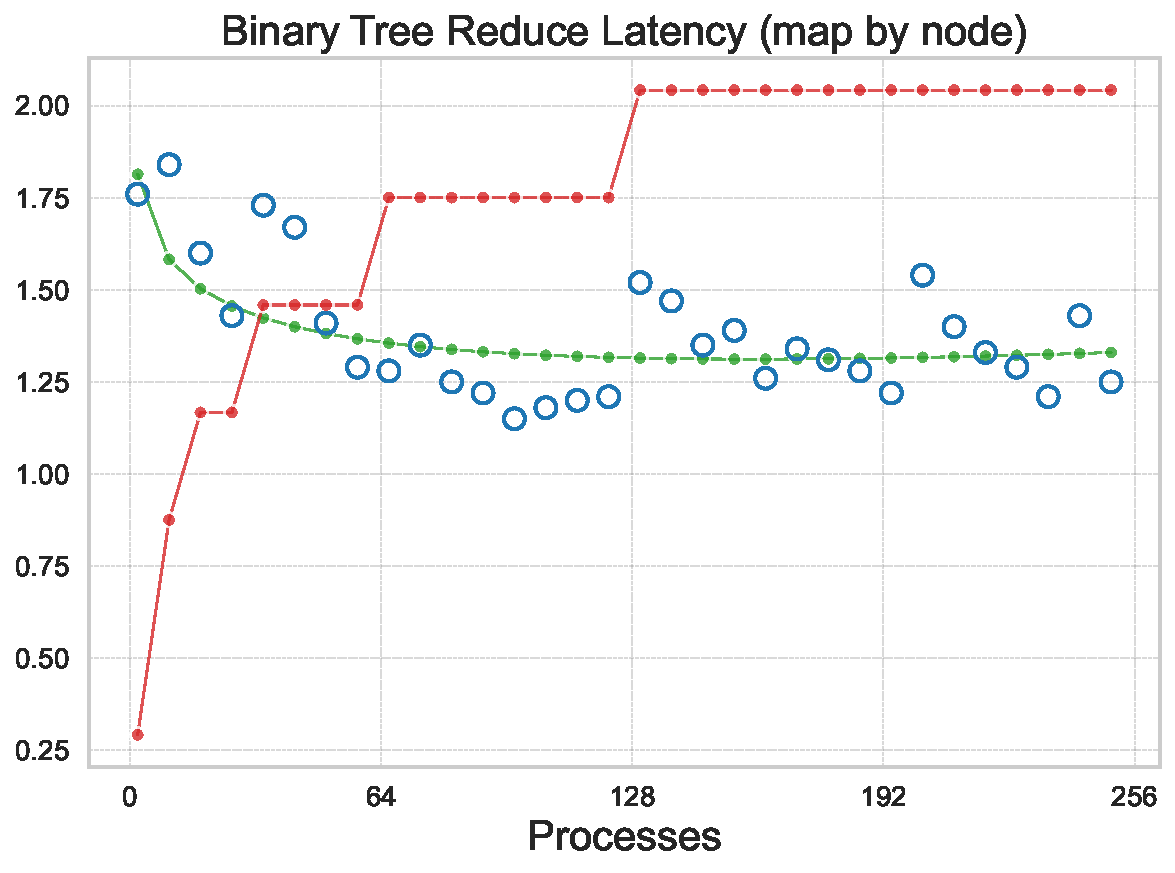
\includegraphics[width=\textwidth]{reduce-binary-node.pdf}
    \end{minipage}
    \end{adjustwidth}
    
    \caption{Comparison between point-to-point and linear fit models for different \textbf{reduce} algorithms and mapping policies. In blue the measured data, corresponding to a message size of $1$ B. The point-to-point model predictions are shown in red while the linear model predictions are shown in green.}
    \label{fig:bcast-results}
\end{figure}

\end{document}
